% Este archivo es parte de la presentación de libWiiEsp, protegida bajo la 
% licencia GFDL. Copyright (C) 2011 Ezequiel Vázquez de la Calle

% -*-planificacion.tex-*-

\section{Planificación temporal}
\begin{frame}
\frametitle{Planificación temporal}
	\begin{block}{Calendario final}
	\noindent Pruebas informales de \emph{Libogc} realizadas durante el curso 09-10.\\
	En noviembre de 2010 se decide construir una biblioteca completa.
	\begin{itemize}
		\item \textbf{Fase de planificación}: realizar pruebas de viabilidad, investigación y búsqueda de información necesaria.
		\item \textbf{Fase de desarrollo}: establecer requisitos y construcción de módulos.
		\begin{itemize}
			\item Por cada módulo:
			\begin{itemize}
				\item Análisis: identificación de funcionalidad necesaria.
				\item Diseño: diseño del componente.
				\item Implementación: codificación del módulo.
				\item Pruebas: comprobaciones y validaciones.
			\end{itemize}
			\item Construcción de juegos de ejemplo.
		\end{itemize}
	    \item \textbf{Fase de documentación}: redactar manual, referencia y memoria del proyecto.
	\end{itemize}
	\end{block}
\end{frame}

\begin{frame}
\frametitle{Diagrama de Gantt}
	\begin{figure}[H]
		\label{gantt}
		\begin{center}
		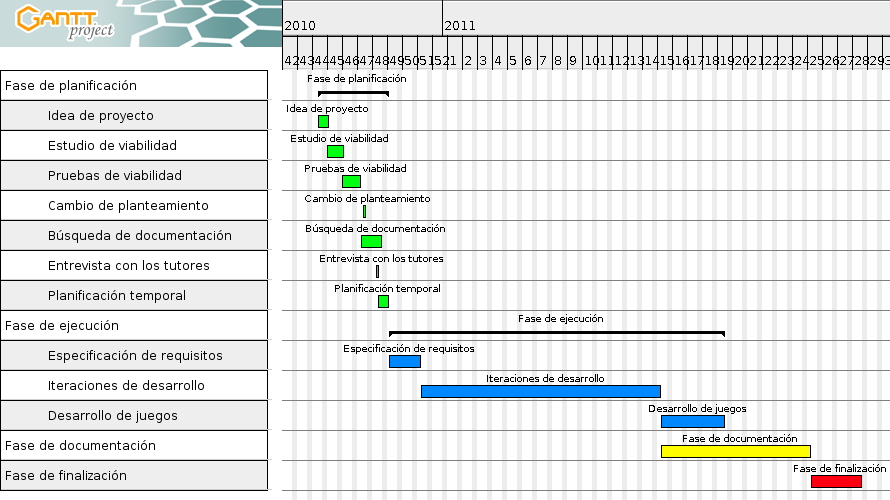
\includegraphics[scale=0.33]{gantt.png}
		\end{center}
		\caption{Diagrama de Gantt}
	\end{figure}
\end{frame}

